\documentclass[11pt]{article}
% /usr/local/texlive/2013/bin/x86_64-darwin/pdflatex 
\usepackage[T1]{fontenc}
\usepackage[utf8]{inputenc}
\usepackage[fleqn]{amsmath}
\usepackage{amssymb}
\usepackage{graphicx}
\usepackage{hyperref}
\usepackage{parskip}
\usepackage{tikz} 
\usepackage{wrapfig} 
\usepackage{alltt}

\renewcommand{\ttdefault}{txtt}

\usepackage[letterpaper]{geometry}
\linespread{1.5}
\usepackage[font=small,labelfont=bf]{caption}
%\usepackage{cancel}

% körper und mengen
\newcommand{\setn}{\mathbb N}
\newcommand{\setr}{\mathbb R}
\newcommand{\setc}{\mathbb C}
\newcommand{\setk}{\mathbb K}

% reihe von #1 bis unendlich über #2
\newcommand{\reihe}[2]{\sum\limits_{#1}^{\infty}{#2}}
% summe von #1 bis #2 über #3
\newcommand{\summe}[3]{\sum\limits_{#1}^{#2}{#3}}
% integral von #1 bis #2 über #3 nach #4
\newcommand{\integrald}[4]{\int\limits_{#1}^{#2}{#3 \; \mathrm d#4}}
% integral von #1 bis #2 über #3 (d/dx muss dann selbst angegeben werden)
\newcommand{\integral}[3]{\int\limits_{#1}^{#2}{#3}}
% integralberechnung von #1 bis #2 über 3
\newcommand{\integralv}[3]{\left[ #3 \right]_{#1}^{#2}}
% betrag mit wachsenden betragsstrichen
\newcommand{\betrag}[1]{\left| #1 \right|}
% limes n gegen unendlich
\newcommand{\limesn}[1]{\lim\limits_{n \to \infty}{#1}}
% limes h gegen 0
\newcommand{\limesh}[1]{\lim\limits_{h \to 0}{#1}}
% vektor kurzschreibweise...
\newcommand{\vect}[1]{\left(\begin{array}{c}#1\end{array}\right)}
%normen
\newcommand{\norm}[1]{\left \Vert {#1} \right \Vert}
\newcommand{\normzwei}[1]{\norm {#1}_{2}}
\newcommand{\norminfty}[1]{\norm {#1}_{\infty}}
\newcommand{\qed}{\hfill \ensuremath{\Box}}
% namentabelle till lukas stefan
\newcommand{\lukas}{\begin{center}
	\begin{tabular}{c|c}
		Name & Student ID \\
		\hline
		Lukas Pfahler & 577332 \\
	\end{tabular}
\end{center}}
% gruppe
\newcommand{\gruppe}[1]{\begin{center} Gruppe {#1} \end{center}}

\title{Information Retrieval and Web Search - Project Phase 2}
\author{Lukas Pfahler \and Tejas Umakanth}
\begin{document}
\maketitle
\section{Collaboration Details}	
	Lukas implemented the web interface, the lucene search engine backend and the hadoop backend including the ranking algorithm used for hadoop search. Tejas implemented the mapreduce jobs that created the index json files.
\section{Architecture}
	\subsection{Indexing}
	\subsection{Webinterface and Search Engine}
		\begin{figure}[h]
			\begin{center}
				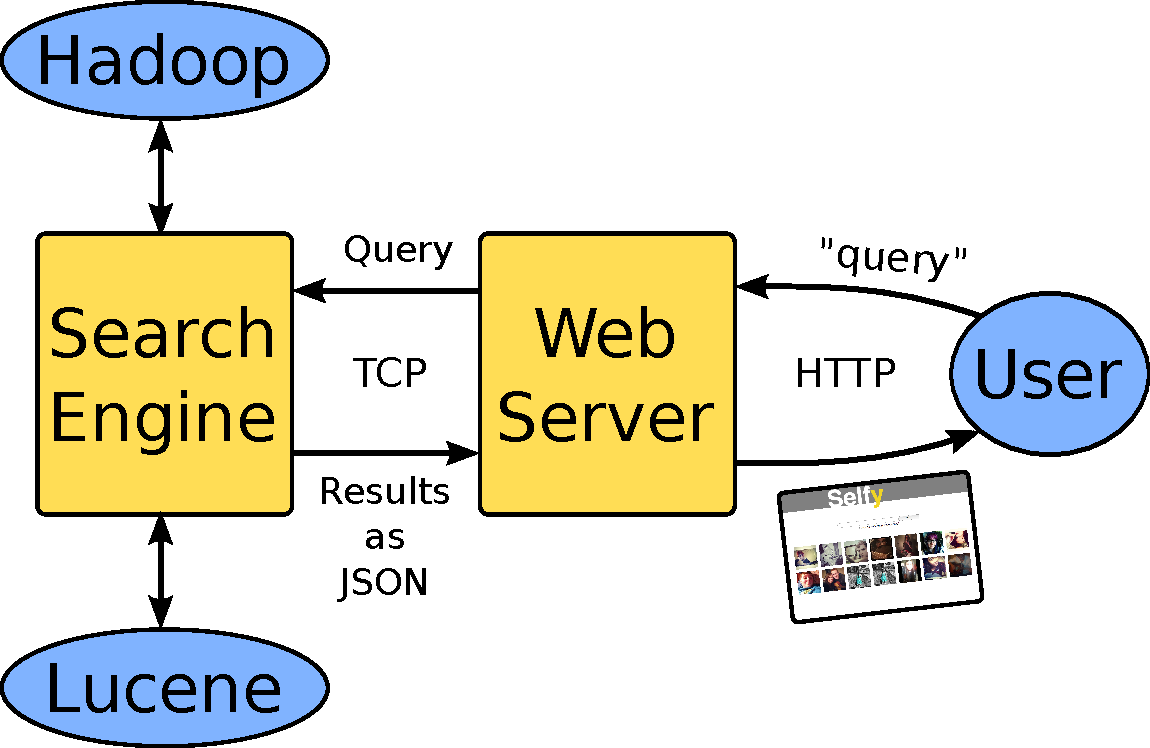
\includegraphics[width=0.9\textwidth,keepaspectratio]{architecture.pdf}
			\end{center}
			\caption{An overview of our search engine architecture.}
			\label{fig1}
		\end{figure}
		For the web interface we decided to go with node.js again. We start a http server on port 80 and wait for requests. Once a user enters a query, our webserver opens a TCP connection to our searchengine backbone, specifying whether to use Lucene or Hadoop and relaying the query. The backbone executes the query and returns the results as JSON. The resultsare then  output to the user by the webserver. Additional information about the documents is loaded in an asynchronus fashion using AJAX and JSON.
	\subsection{Searching}


\section{Usage}
	\subsection{Crawler}
		To run our crawler, you first have to install node.js, which you can download at 
		\begin{center}{\vspace{-3mm}\url{http://nodejs.org/download/}}\end{center}
		We are also using the request node-module, which you can download and install by running the following command:
		\begin{alltt}
			npm install request
		\end{alltt}
		Now you can run our crawler by calling
		\begin{alltt}
			node instagramStream.js
		\end{alltt}
		which will start a http-server on port 1337 of your local machine. Please note that port 1337 of your machine has to be open to the public. To actually start crawling, you have to subscribe to instagram media updates. This is done by calling the following command:
		\begin{alltt}
			curl -F 'client_id=620c46f7e7da46149b0ad5d3cd8268ba' \textbackslash 
			     -F 'client_secret=c57beab5c2864e608b0dc4e46e5f8b50' \textbackslash
			     -F 'object=tag' -F 'aspect=media' -F 'object_id=\textbf{selfie}' \textbackslash
			     -F 'callback_url=\{http://\textbf{YOUR_IP}:1337\}' \textbackslash
			     https://api.instagram.com/v1/subscriptions/
		\end{alltt}
		This will subscribe to all updates of the (very popular) hashtag $\#$selfie; the crawler will start storing media items in a newly created folder selfies.

		You can unsubscribe from updates by running
		\begin{alltt}
			curl -X DELETE 'https://api.instagram.com/v1/subscriptions?client_secret=\textbackslash
			     c57beab5c2864e608b0dc4e46e5f8b50&object=all&\textbackslash
			     client_id=620c46f7e7da46149b0ad5d3cd8268ba'
		\end{alltt}

		You should always unsubscribe before shutting down the crawler (\texttt{CTRL-C}), if you fail to do so you might not be able to subscribe to media for a while. We suspect that the servers at Instagram need some time to realize that our crawler is not running anymore and continue to try to send the new subscriptions to our already shutdown crawler.
	\subsection{Indexer}
		To deploy our indexer, you have to execute the jar file by typing 
		\begin{alltt}
			java -jar indexer.jar \textbf{\{datadir\}}
		\end{alltt}
		An ‘index’ folder will be created in the file containing the all the files of the project.

\section{Performance}
	The time needed to for indexing is dependent on the system on which the indexing is done. This performance analysis was carried out on a laptop with a 2.4 GHz CPU. For performing this test, we use a document containing 3GB worth of JSON files that are returned by our crawler. Then we try to index the JSON files in the document and calculate the time taken to index. As we can see in figure 1, the indexing time increases almost linearly as the number of JSON files that are indexed increases.
	\begin{figure}
		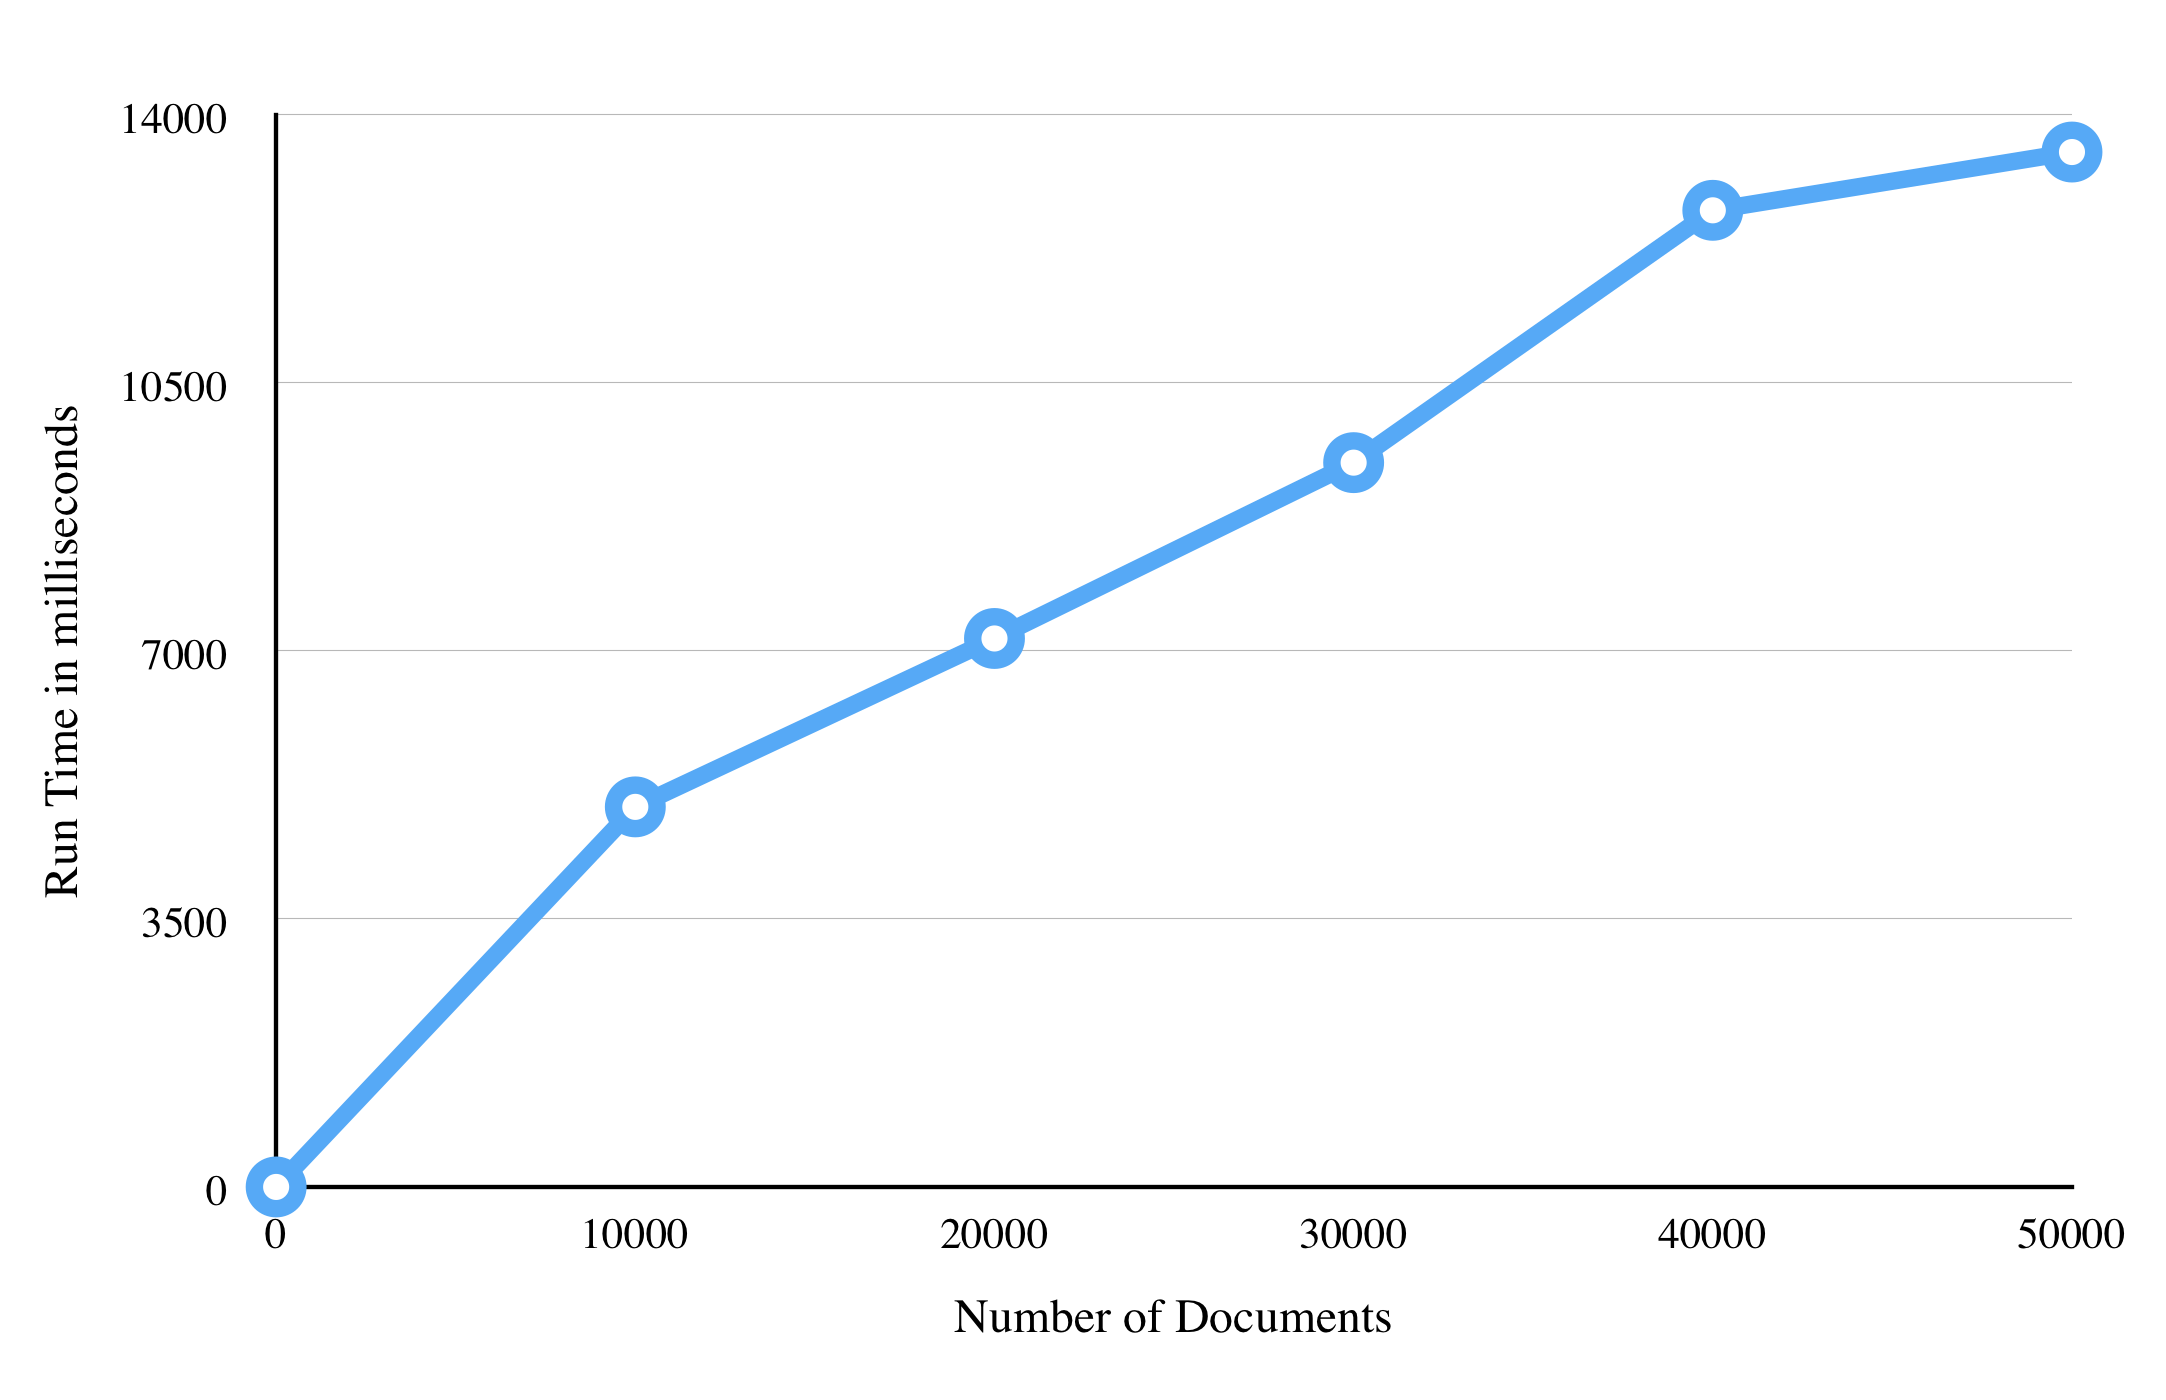
\includegraphics[keepaspectratio, width=\textwidth]{Chart.pdf}
		\caption{Indexing Performance}
		\label{fig:1}
	\end{figure}
\section{Screenshots}

\end{document}
